%% \documentclass{report}
%% \usepackage{fullpage}
%% \usepackage{tikz}
%% \usepackage[utf8]{inputenc}
%% \usepackage[OT1]{fontenc}

%% \begin{document}

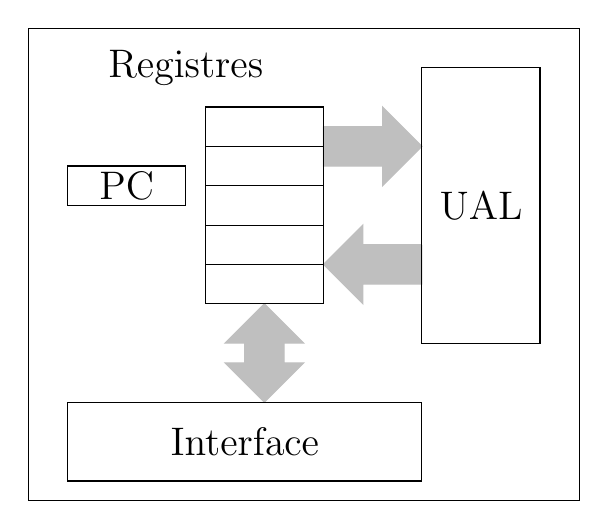
\begin{tikzpicture}

\newcommand{\myarrowright}[3]{% x depart, y depart, longueur
\draw[black!25,fill=black!25] (#1,#2+0.25) -- (#1+#3-0.5,#2+0.25) -- (#1+#3-0.5,#2+0.5) -- (#1+#3,#2) -- (#1+#3-0.5,#2-0.5) -- (#1+#3-0.5,#2-0.25) -- (#1,#2-0.25) -- (#1,#2+0.25);
}
\newcommand{\myarrowleft}[3]{% x depart, y depart, longueur
\draw[black!25,fill=black!25] (#1,#2+0.25) -- (#1-#3+0.5,#2+0.25) -- (#1-#3+0.5,#2+0.5) -- (#1-#3,#2) -- (#1-#3+0.5,#2-0.5) -- (#1-#3+0.5,#2-0.25) -- (#1,#2-0.25) -- (#1,#2+0.25);
}
\newcommand{\myarrowup}[3]{% x depart, y depart, longueur
\draw[black!25,fill=black!25] (#1+0.25,#2) -- (#1+0.25,#2+#3-0.5) -- (#1+0.5,#2+#3-0.5) -- (#1,#2+#3) -- (#1-0.5,#2+#3-0.5) -- (#1-0.25,#2+#3-0.5) -- (#1-0.25,#2) -- (#1+0.25,#2);
}
\newcommand{\myarrowdown}[3]{% x depart, y depart, longueur
\draw[black!25,fill=black!25] (#1+0.25,#2) -- (#1+0.25,#2-#3+0.5) -- (#1+0.5,#2-#3+0.5) -- (#1,#2-#3) -- (#1-0.5,#2-#3+0.5) -- (#1-0.25,#2-#3+0.5) -- (#1-0.25,#2) -- (#1+0.25,#2);
}


%% \foreach \i in {0,...,15} {
%%   \foreach \j in {-20,...,0} {
%%     \node[black!25] at (\i,\j) {\i,\j};
%%   }
%% }

%cpu
\draw (0,0) rectangle (7,-6);
%\node at (8.25,-0.25) {\Large Processeur};
%bus registers->ALU
\myarrowright{3.75}{-1.5}{1.25}
%bus ALU->registers
\myarrowleft{5}{-3}{1.25}
%bus interface->registers
\myarrowup{3}{-4}{0.5}
%registers->bus interface
\myarrowdown{3}{-4}{0.75}
%pc
\draw (0.5,-1.75) rectangle (2,-2.25);
\node at (1.25,-2) {\Large PC};
%other registers
\draw (2.25,-1) rectangle (3.75,-3.5);
\draw (2.25,-1.5) -- (3.75,-1.5);
\draw (2.25,-2) -- (3.75,-2);
\draw (2.25,-2.5) -- (3.75,-2.5);
\draw (2.25,-3) -- (3.75,-3);
\node at (2,-0.5) {\Large Registres};
%alu
\draw (5,-0.5) rectangle (6.5,-4);
\node at (5.75,-2.25) {\Large UAL};
%bus interface
\draw (0.5,-4.75) rectangle (5,-5.75);
\node at (2.75,-5.25) {\Large Interface};

\end{tikzpicture}

%\end{document}
